\chapter{Trajectory Planning}%
\label{CH:PLANNING}

%----------------------------------------------------------------------------------------
\section{The Framework}
In the previous chapter, we tracked the problem of autonomous environment \emph{exploration} from a very practical point of view,
providing a couple of possible solutions to efficiently compute high informative trajectories. Here, we moved to a slightly different
problem as the environment to navigate is completely known and the main objective is to move the autonomous agent from an initial
position, to a final one, without getting in collision with the mapped obstacles and without the necessity to gather information about
the surroundings. In these settings, the planned trajectory is required only to be \emph{safe} in the sense that does not collide with
any obstacles and develops inside known and free environment areas, and to fully satisfy the agent dynamical capabilities.
As the trajectory is not meant to gather as much data as possible, it can be designed to optimise whatever user-defined loss function,
from the overall travel time, to control effort, or high derivatives. In the Leonardo drone contest case, a trajectory planning module
was required to navigate the environment and reach a goal position smoothly and quickly, so the quadrotor is steered in a way that
the localisation and the collision avoidance (see later in~\chref{CH:AVOIDANCE}) parts can work as well as possible.

In this chapter, after a brief literature review, we analyze and adapt a state-of-the-art solution to the trajectory planning problem.
The proposed solution has been successfully implemented and deployed during the Leonardo drone contest.
For further details the reader is referred to the original work~\cite{zhou2019robust}.

\subsection{Related Works}
Although the literature is cluttered of possible solutions to the problem at hand, most of them can be classified solely in two
categories: \emph{hard constrained} and \emph{soft costrained} methods.
Hard constrained methods reformulate the trajectory planning as a convex optimisation problem, this idea 
is pioneered by~\cite{mellinger2011minimum} that proposes to generate minimum-snap trajectories
via Quadratic Programming (QP) approach, and by~\cite{richter2016polynomial} that, in turn, presented a closed-form approach
to the minimum-snap trajectory generation problem.
Both the latter approaches parametrise the overall trajectory as $n$-segments piecewise polynomial curve,
and ensure the trajectory safety by iteratively adding intermediate waypoints.
Similar approaches generate safe trajectories via convex optimisation~\cite{chen2015real, gao2016online, liu2017planning, ding2018trajectory, ding2019efficient, gao2018online},
unlike the pioneer solutions, here the problem is solved in a two-steps pipeline. First, a sequence of cubes~\cite{gao2018online},
or spheres~\cite{gao2019flying}, or polyhedrons~\cite{liu2017planning}, are fitted inside the free and navigable space, then the
reconstructed flight corridors are used as convex constraints inside the optimisation problem.
The works~\cite{ding2018trajectory, ding2019efficient} proposed a B-Spline-based search able to generate trajectories used as 
initial guess for the subsequent optimisation step.
Thanks to the convex reformulation, hard constrained methods guarantee global optimality at exspense of all possible nonconvex
costs and constraints, such as distance from obstacles and conservative kinodynamic constraints.
On the other hand, soft constrained methods reformulate the trajectory planning as a non-linear optimisation problem able to keep
safety into account, 


There are also methods for- mulating trajectory generation as a non-linear optimization problem that takes smoothness
and safety into account. 

\cite{zucker2013chomp} generates discrete-time trajectories by minimizing its smooth- ness and collision costs
using gradient descent methods. 
\cite{kalakrishnan2011stomp} has similar problem formulation, but the optimization is solved by a gradient-free
sampling method. 

\cite{oleynikova2016continuous} extended them to continuous-time polynomial trajectories. Since the time pa- rameterization is continuous,
it avoids numeric differentiation errors and is more accurate to represent the motions of quadrotors. However, it suffers from
a low success rate. To solve this problem, \cite{gao2017gradient} finds a collision-free initial path firstly using an
informed sampling-based path searching method. This path serves as a higher quality initial guess of

non-linear optimization and thus improve the success rate. In \cite{usenko2017real}, the trajectory is parameterized as a uniform B-spline.
Since a B- spline is continuous by nature, there is no need to enforce
continuity explicitly, which reduce the number of constraints.
It is also particularly useful for local replanning thanks to its property of locality.
Soft-constrained methods utilize gradient information to push trajectory far from obstacles,
but suffer from local minima and having no strong guarantee of success rate and kinodynamic feasibility.
Our optimization method also utilizes gradient information to improve the safety of the trajectory.
However, unlike previous methods in which computational expensive line integrals along the trajectory are calculated,
the formulation is redesigned to be simpler based on the convex hull property of B-spline.
It greatly improves the computation efficiency as well as the convergent rate.

%----------------------------------------------------------------------------------------
\section{Quadrotor Trajectory Generation}

\subsection{Hybrid State A$^{\star}$}
\subsection{Trajectory Optimisation}
\subsection{Experimental Results}

%----------------------------------------------------------------------------------------
\section{Contributions}

\begin{figure}[!t]
	\begin{center}
		\begin{minipage}{.45\linewidth}
			\centering
			\subfloat[]{%
				\label{FIG:PLANNING-RESULTS-MAP-TRAJECTORY-A}%
				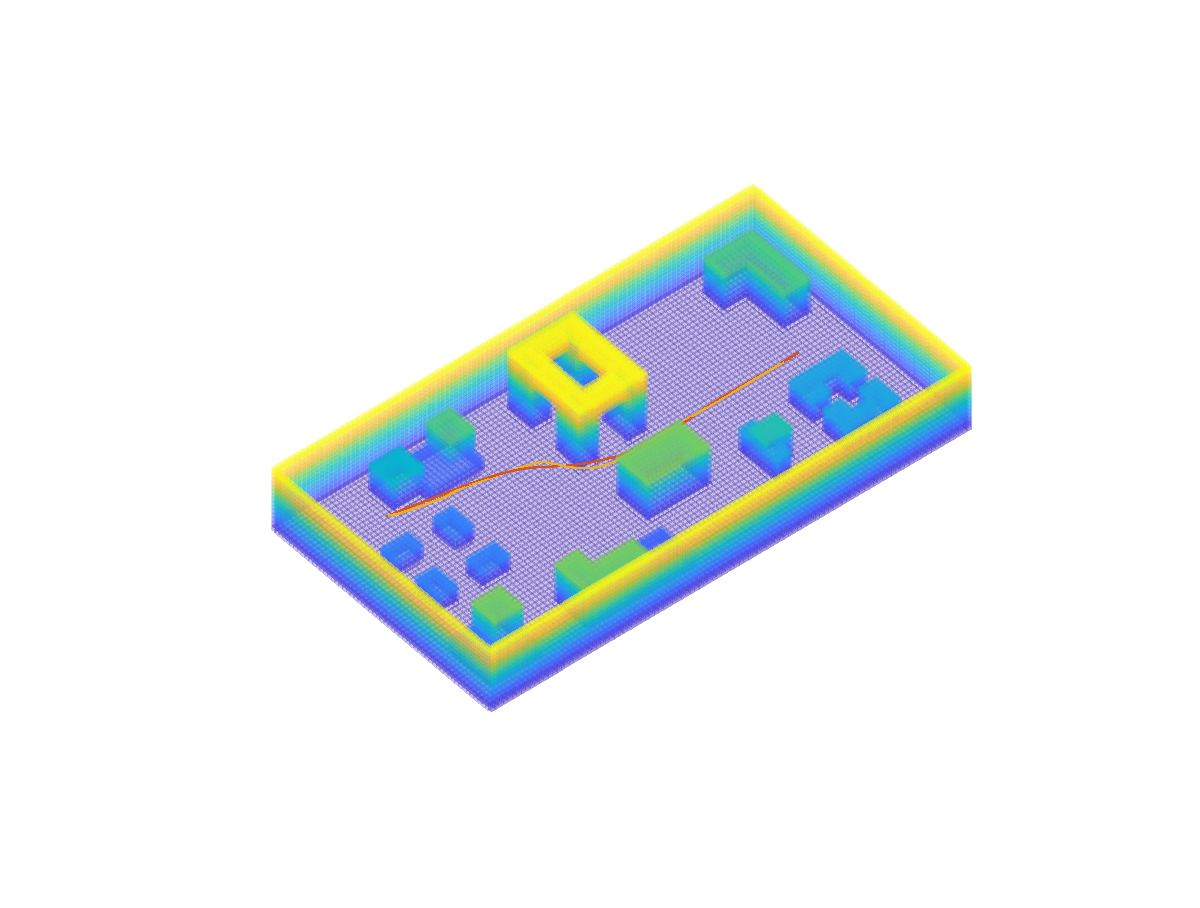
\includegraphics[trim={3.5cm 2.5cm 3cm 2.5cm}, clip = true, width = 1.05\textwidth]{Figs/Chapter5/planning-full.eps}}
		\end{minipage}
		\begin{minipage}{.45\linewidth}
			\centering
			\subfloat[]{%
				\label{FIG:PLANNING-RESULTS-MAP-TRAJECTORY-B}%
				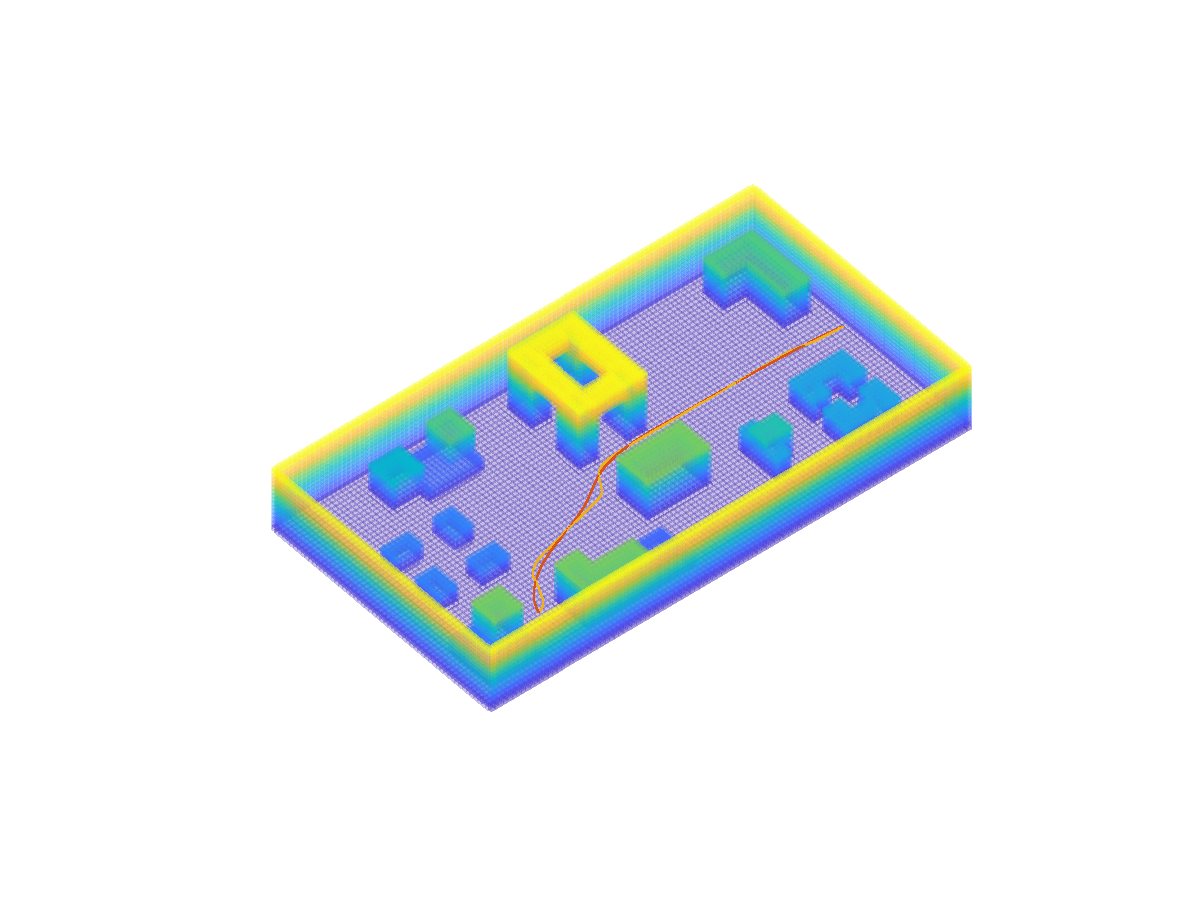
\includegraphics[trim={3.5cm 2.5cm 3cm 2.5cm}, clip = true, width = 1.05\textwidth]{Figs/Chapter5/planning-full-2.eps}}
		\end{minipage}
	\end{center}
	\caption{Caption here.}%
    \label{FIG:PLANNING-RESULTS-MAP-TRAJECTORY}
\end{figure}

\begin{figure}[!t]
	\begin{center}
		\begin{minipage}{.45\linewidth}
			\centering
			\subfloat[]{%
				\label{FIG:PLANNING-RESULTS-TRAJECTORY-A}%
				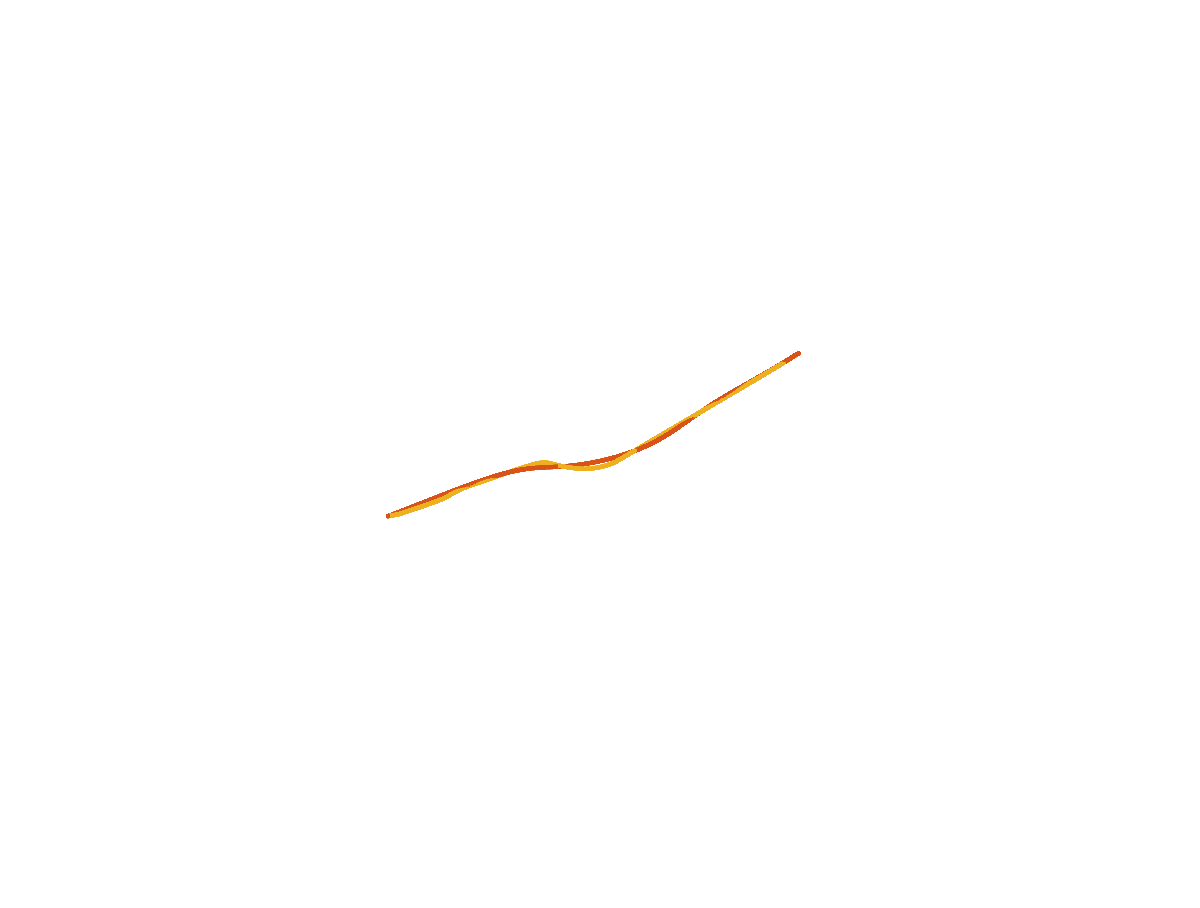
\includegraphics[trim={3.5cm 2.5cm 3cm 2.5cm}, clip = true, width = 1.05\textwidth]{Figs/Chapter5/planning-traj.eps}}
		\end{minipage}
		\begin{minipage}{.45\linewidth}
			\centering
			\subfloat[]{%
				\label{FIG:PLANNING-RESULTS-TRAJECTORY-B}%
				
\includegraphics[trim={3.5cm 2.5cm 3cm 2.5cm}, clip = true, width = 1.05\textwidth]{Figs/Chapter5/planning-traj-2.eps}}
		\end{minipage}
	\end{center}
	\caption{Caption here.}%
    \label{FIG:PLANNING-RESULTS-TRAJECTORY}
\end{figure}

%------------------------------------------------